
%% 1-2 pages

\section{Related research}
This section presents the research upon which this study builds.

TODO: Update this section with more focus on technical debt rather than information visualization.

The core of information visualizations are the mapping of data and intent to visual representations. Although there are many different techniques used in the field, this central process of visualizations can be described by the \textit{Reference model for visualization} by Card et al. presented in figure \ref{fig:vizprocess}. \cite{card_readings_1999} 
This common reference model is helpful in order to analyze and compare the different techniques as seen in the taxonomy proposed by Chi based on model by Card et al. \cite{chi_taxonomy_2000}

\begin{figure}[t]
  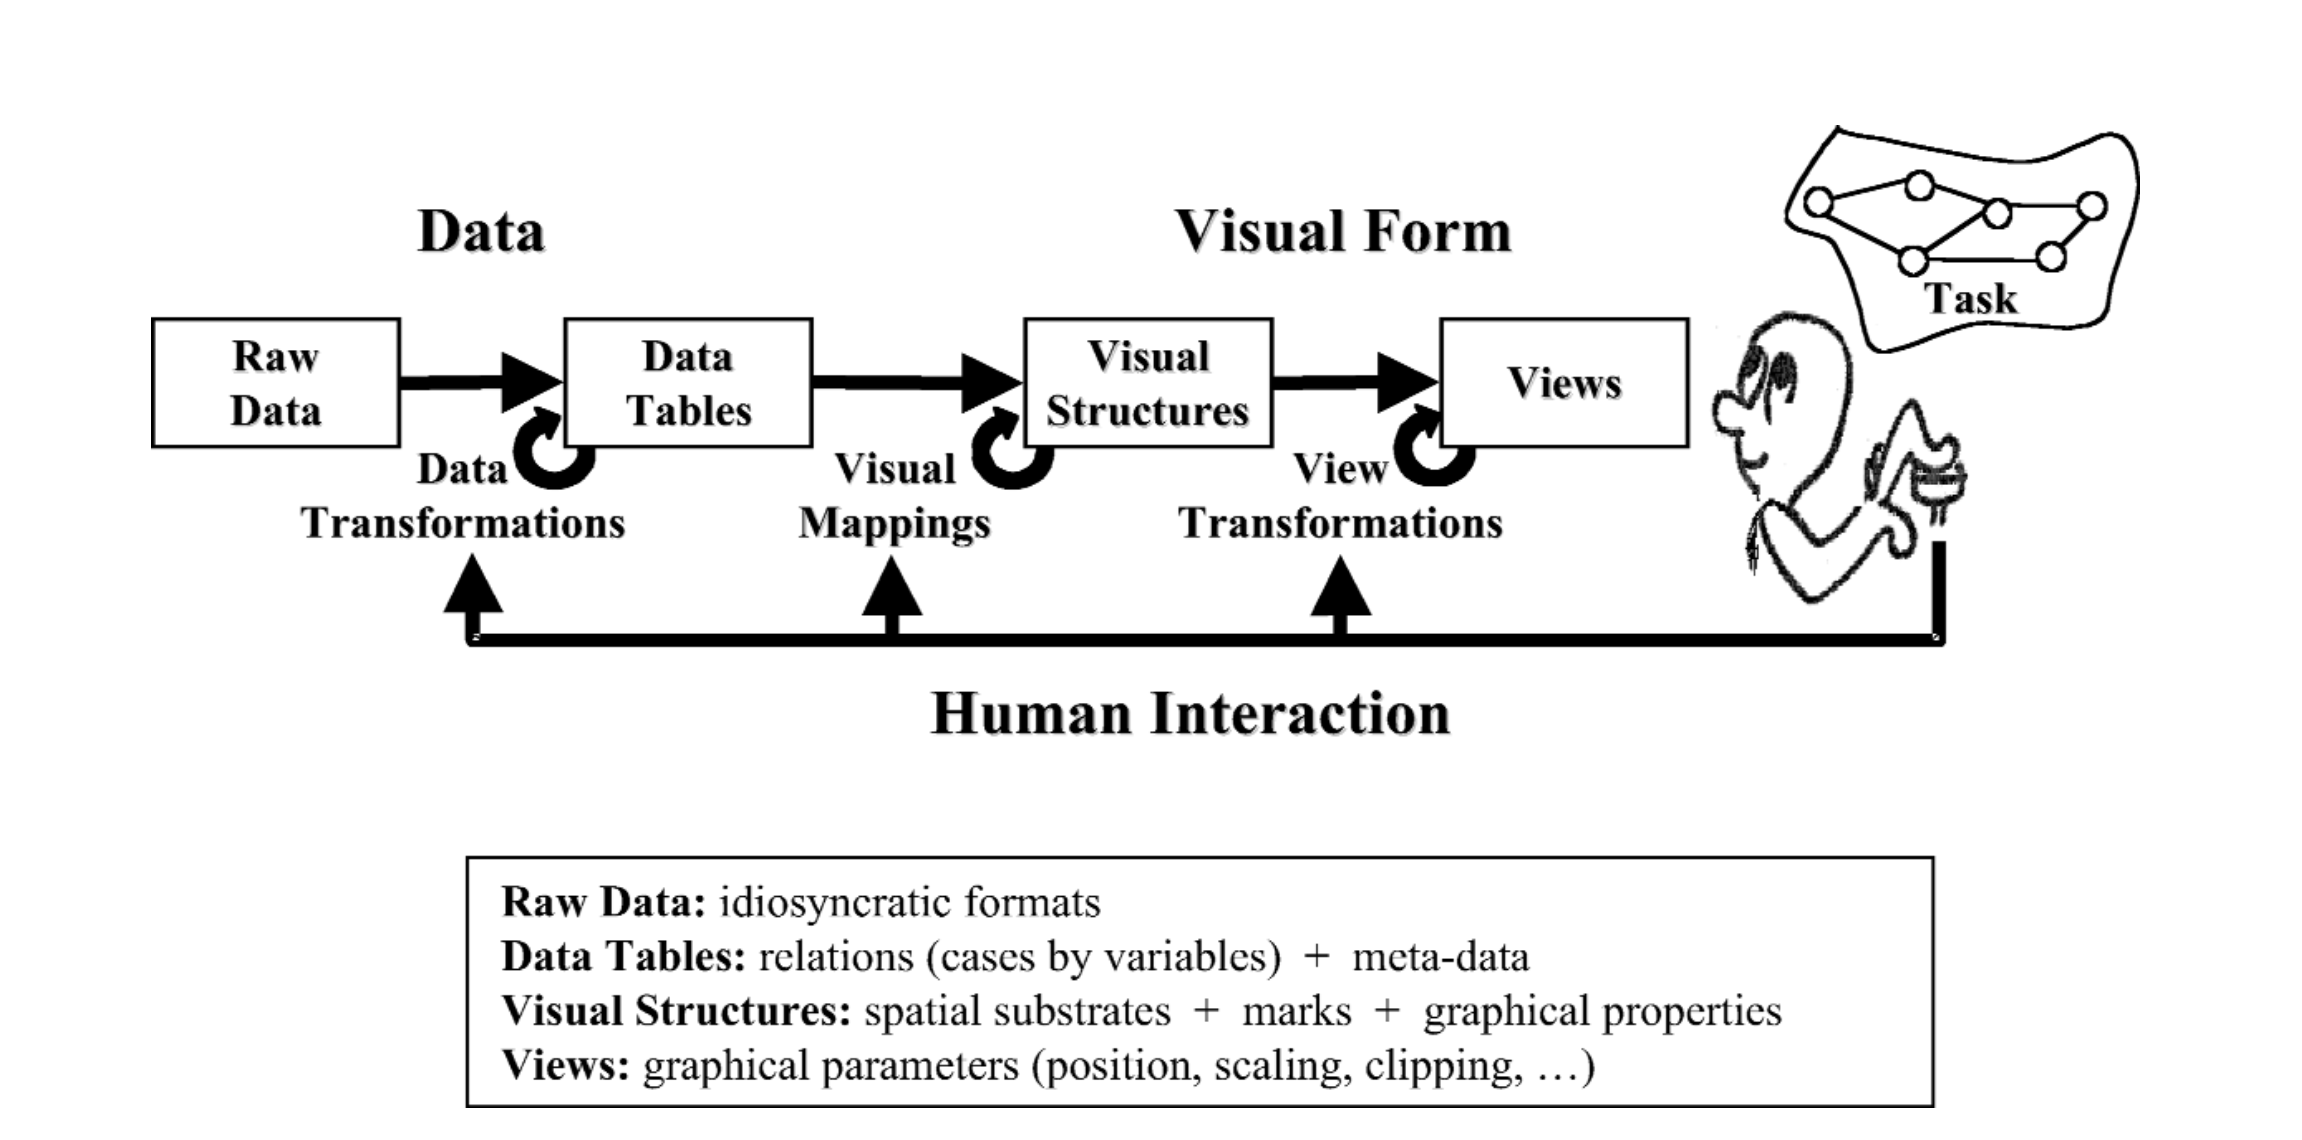
\includegraphics[width=\columnwidth]{VisualizationProcess}
  \Description{Chart over the Reference model for visualization by Card et al. 1999}
  \caption[Reference model for visualization]{Reference model for visualization by Card et al. 1999 \cite{card_readings_1999}}.
  \label{fig:vizprocess}
  \centering
\end{figure}

The raw data can take many forms which can be classified intro three main categories based on its properties, \textit{nominal data} is simple data with some sort of label but no quantitative value, \textit{ordinal data} can be ranked according to some attribute and \textit{quantitative data} which support arithmetic operations. \cite{card_structure_1997}

Previous research has been published investigating software evolution through different visualization techniques. 


Bayer and Hassan developed "Evolution Storyboards"


, examples include code-swarm, CVSscan and Software evolution storylines. However, during the last decade tools and workflows used by software development teams have evolved and more information is recorded with every change, allowing for rich analyses of the history and evolution of software source code.

The previous work mentioned contributed with valuable knowledge and in doing that also created new questions to be answered.
In comparison to CVSscan which focuses on single files, this thesis will investigate a whole repository of source code to give a better overview and richer understanding about how the whole projects evolves.
code-swarm and Software evolution storylines presented intuitive visual mappings for data points but targeted casual users and did not allow for interaction and deeper exploration of the data.
In contrast, this study targets advanced users with domain knowledge and information about the context of the software project, allowing for a more advanced interactive visualization tool that presents complex information.
